\section{电路设计}
\subsection{电路分类}
\begin{enumerate}
\item 摩尔(Moore)电路
\begin{figure}[htbp]
	\centering
	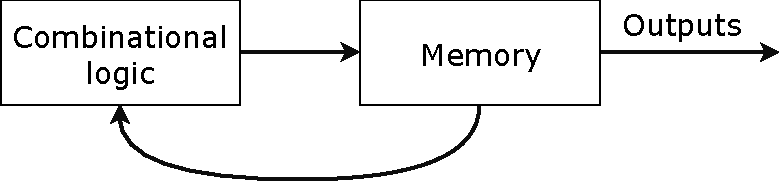
\includegraphics[width=0.4\linewidth]{fig/moore_machine.pdf}
	\caption{触发器}
\end{figure}
\item 米勒(Mealy)电路
\begin{figure}[htbp]
	\centering
	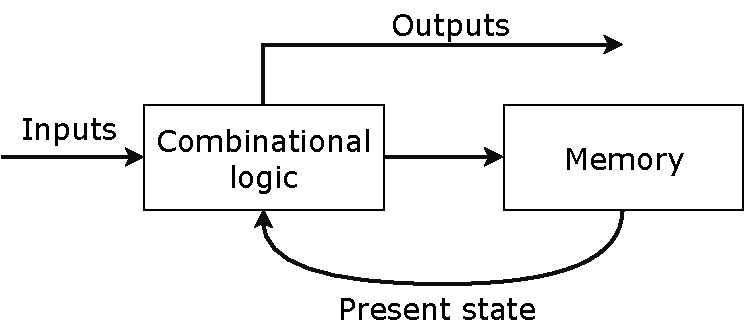
\includegraphics[width=0.4\linewidth]{fig/mealy_machine.pdf}
	\caption{触发器}
\end{figure}
\end{enumerate}
\subsection{设计步骤}
\par 基于状态转移表格的方法
\begin{enumerate}
    \item 状态图
    \item 次态表
    \item 触发器转移表
\begin{center}
\begin{tabular}{|c|c|c|c|}
\hline
$Q^n$ & $Q^{n+1}$ & J & K\\\hline
0 & 0 & 0 & X\\\hline
0 & 1 & 1 & X\\\hline
1 & 0 & X & 1\\\hline
1 & 1 & X & 0\\\hline
\end{tabular}
\end{center}
    \item 触发器JK卡诺图
    \item JK驱动方程
    \item 时序电路
\end{enumerate}
\par 基于状态方程的方法
\begin{enumerate}
	\item 状态表
	\item 次态卡诺图
	\item 状态方程 $Q^{n+1}=J\ol{Q^n}+\ol{K}Q^n$
	\item 驱动方程
	\item 时序电路
\end{enumerate}
\subsection{实例操作}
\par 目的:用JK触发器实现一个12进制同步计数器
\begin{enumerate}
    \item 状态转换图
    \begin{figure}[H]
        \centering
        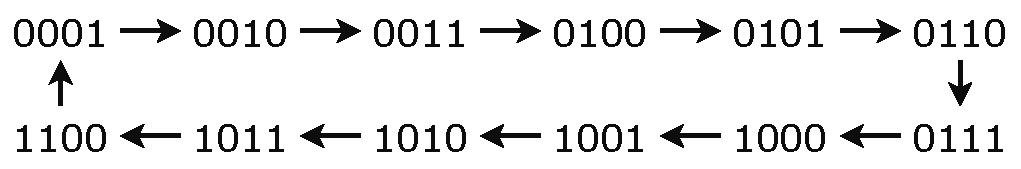
\includegraphics[width=0.7\linewidth]{fig/12system_state.pdf}
    \end{figure}
    \item 确定电路所需触发器数目\\
    由于$2^4=16>12$,故需要$4$个JK触发器
    \item 次态卡诺图
    \begin{figure}[H]
        \centering
        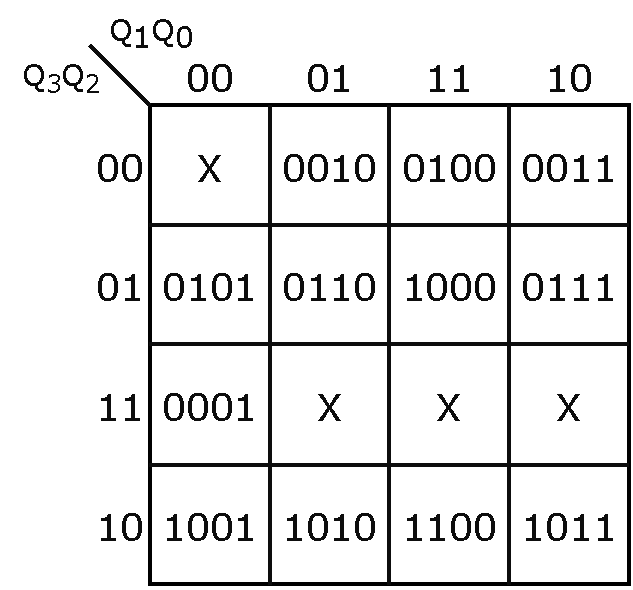
\includegraphics[width=0.4\linewidth]{fig/Karnaugh_12system.pdf}
    \end{figure}
    \item 触发器状态方程,由卡诺图可得
    \[\begin{aligned}
    Q_0^{n+1}&=\overline{Q_0}\\
    Q_1^{n+1}&=Q_0\overline{Q_1}+\overline{Q_0}Q_1\\
    Q_2^{n+1}&=Q_0Q_1\ol{Q_2}+\ol{Q_1}Q_2\ol{Q_3}+\ol{Q_0}Q_2\ol{Q_3}\\
    Q_3^{n+1}&=\ol{Q_2}Q_3+Q_0Q_1Q_2\ol{Q_3}
    \end{aligned}\]
    \item 触发器驱动方程,由
    \[Q^{n+1}=J\ol{Q^n}+\ol{K}Q^n\]
    将状态方程整理为上式形式,可得
    \[\begin{aligned}
    J_0&=1 \qquad &K_0&=1\\
    J_1&=Q_0 \qquad &K_0&=Q_0\\
    J_2&=Q_1Q_0 \qquad &K_2&=\ol{\ol{Q_3}\ol{Q_1}+\ol{Q_3}\ol{Q_0}}=\ol{Q_3}+Q_1Q_0\\
    J_3&=Q_2Q_1Q_0 \qquad &K_3&=Q_2
    \end{aligned}\]
    \item 检查自启动\\
    当输入为1111和0000时,可自动跳转至0001;输入为1101时,跳转至0010;输入为1110时,跳转至0011
\end{enumerate}
\par Proteus电路图连接如下
\begin{figure}[H]
    \centering
    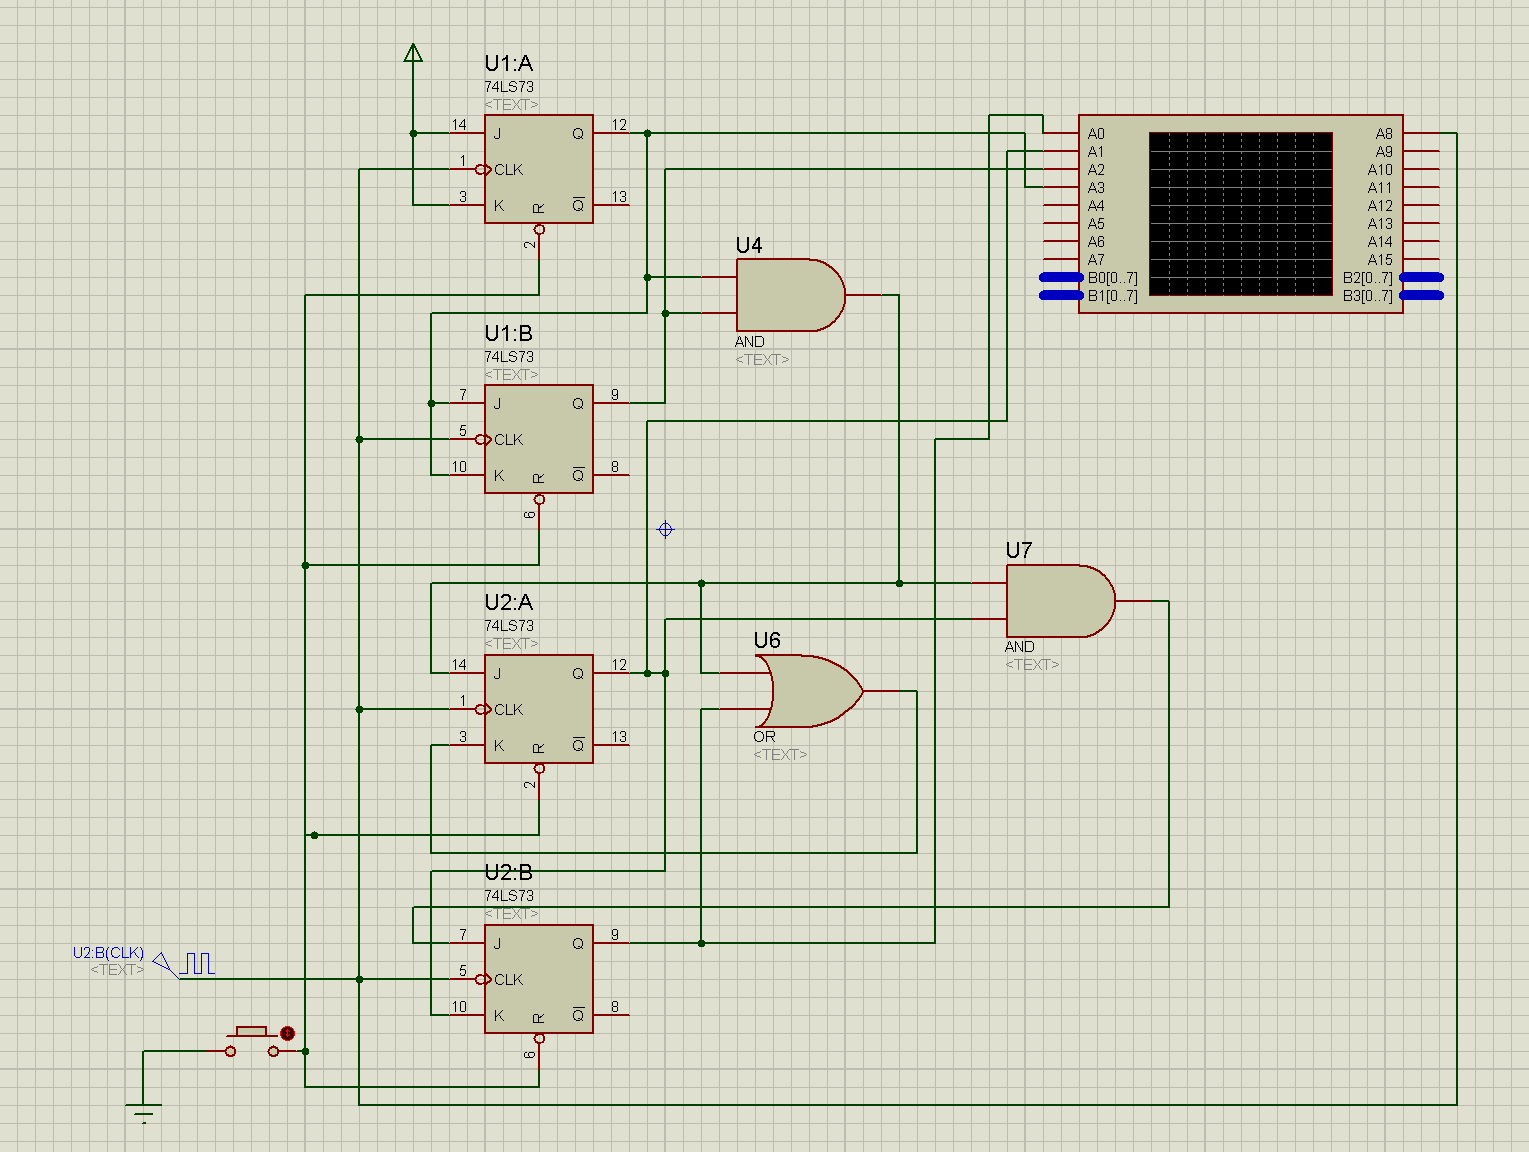
\includegraphics[width=0.9\linewidth]{fig/12system_protues.PNG}
\end{figure}
\par 仿真结果如下
\begin{figure}[H]
    \centering
    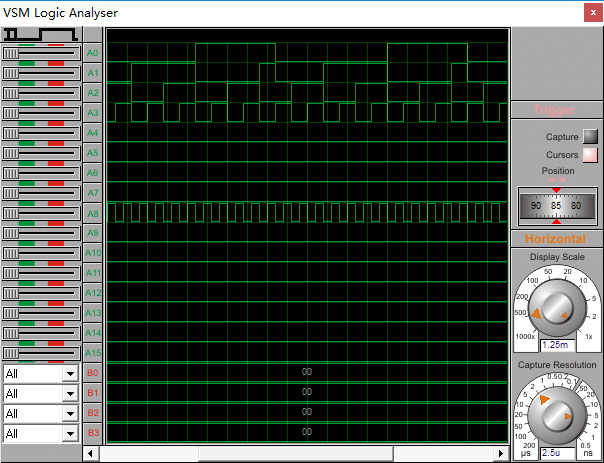
\includegraphics[width=0.6\linewidth]{fig/12system_wave.PNG}
\end{figure}